%%%%%%%%%%%%%%%%%%%%%%%%%%%%%%%%%%%%%%%%%%%%%%%%%%%%%%%%%%%%%%%%%%%%%%
% Template para artigos da SBC
% Adaptado para o trabalho prático de Processamento de Dados com Grafos
%%%%%%%%%%%%%%%%%%%%%%%%%%%%%%%%%%%%%%%%%%%%%%%%%%%%%%%%%%%%%%%%%%%%%%

\documentclass[12pt]{article}

\usepackage{sbc-template}
\usepackage{graphicx,url}
\usepackage[utf8]{inputenc}
\usepackage{amsmath} % Para ambientes matemáticos
\usepackage{listings} % Para blocos de código
\usepackage{xcolor} % Para cores no código

% Configuração para blocos de código
\definecolor{codegreen}{rgb}{0,0.6,0}
\definecolor{codegray}{rgb}{0.5,0.5,0.5}
\definecolor{codepurple}{rgb}{0.58,0,0.82}
\definecolor{backcolour}{rgb}{0.95,0.95,0.92}

\lstdefinestyle{customStyle}{
    backgroundcolor=\color{backcolour},
    commentstyle=\color{codegreen},
    keywordstyle=\color{magenta},
    numberstyle=\tiny\color{codegray},
    stringstyle=\color{codepurple},
    basicstyle=\ttfamily\footnotesize,
    breakatwhitespace=false,
    breaklines=true,
    captionpos=b,
    keepspaces=true,
    numbers=left,
    numbersep=5pt,
    showspaces=false,
    showstringspaces=false,
    showtabs=false,
    tabsize=2
}
\lstset{style=customStyle}

\sloppy

\title{Gestão de Dependências em Projetos Go com Ordenação Topológica}

% TODO: PREENCHER OS DADOS DOS AUTORES E INSTITUIÇÕES
\author{Nicholas Pereira Cristófaro\inst{1}, Nome Sobrenome do Aluno 2\inst{1}}

\address{Pontifícia Universidade Católica de Minas Gerais\\
  Belo Horizonte -- Minas Gerais -- Brasil
  \email{nicholaspcr@gmail.com, email2@dominio.com}
}

\begin{document}

\maketitle

\begin{resumo}
A gestão de dependências é um desafio em software moderno. Este artigo apresenta uma ferramenta que analisa e visualiza dependências em projetos Go, modelando-as como um grafo direcionado. Através da ordenação topológica com o algoritmo de Kahn, a ferramenta determina a sequência de compilação segura e detecta dependências cíclicas — um erro crítico em Go. A solução, implementada em Python, abrange desde a análise do código até a geração de um grafo interativo, oferecendo um suporte prático para a gestão de conflitos em sistemas de dependência.
\end{resumo}

\begin{abstract}
Dependency management is a challenge in modern software. This paper introduces a tool that analyzes and visualizes dependencies in Go projects by modeling them as a directed graph. Through topological sorting with Kahn's algorithm, the tool determines a safe compilation sequence and detects cyclic dependencies—a critical error in Go. The solution, implemented in Python, covers the process from code analysis to generating an interactive graph, providing practical support for managing conflicts in dependency systems.
\end{abstract}

\section{Introdução}


O desenvolvimento de software contemporâneo é caracterizado pela modularidade e reutilização de código, resultando em sistemas compostos por um grande número de componentes interdependentes. A gestão dessa rede de dependências é um desafio central na engenharia de software, por vezes referido como "inferno de dependências" \cite{jergensen2011}. Falhas nesse gerenciamento podem levar a erros de compilação, comportamento inesperado e dificuldades na manutenção.

A linguagem de programação Go (Golang) possui um sistema de pacotes estático e um compilador que impõem regras estritas sobre as dependências. Uma dessas regras é que as dependências de um pacote devem ser inicializadas antes do próprio pacote \cite{donovan2015go}. Isso garante a execução correta das funções \texttt{init()}, que configuram o estado inicial de cada pacote. Quando um projeto contém uma dependência cíclica, o compilador Go gera um erro, pois não é possível determinar uma ordem de inicialização válida \cite{GoSpec}.

A ordem de inicialização de pacotes em Go pode ser modelada como um grafo de dependências direcionado acíclico (DAG). A solução para determinar a sequência correta é, portanto, encontrar uma ordenação topológica desse grafo \cite{clrs}. Este trabalho detalha uma ferramenta que aplica esses conceitos para analisar projetos Go.

Este trabalho se enquadra na proposta de "Gestão de Conflitos em Sistemas de Dependência", focando na modelagem, detecção de ciclos e execução segura baseada em ordenação topológica. Para isso, foi desenvolvida uma ferramenta em Python que:
\begin{itemize}
    \item Analisa recursivamente os arquivos de um projeto Go para extrair as relações de importação.
    \item Constrói um grafo de dependências direcionado a partir dessas relações.
    \item Aplica o algoritmo de Kahn para realizar a ordenação topológica dos pacotes.
    \item Gera uma visualização gráfica do grafo de dependências, destacando a ordem de inicialização em camadas.
\end{itemize}

O restante deste artigo está organizado da seguinte forma: a Seção 2 apresenta a fundamentação teórica sobre grafos, ordenação topológica e o sistema de pacotes do Go. A Seção 3 detalha a modelagem do problema e a arquitetura da ferramenta desenvolvida. A Seção 4 apresenta os experimentos realizados e discute os resultados obtidos. Finalmente, a Seção 5 conclui o trabalho e aponta direções para desenvolvimentos futuros.

\section{Fundamentação Teórica}
Esta seção aborda os conceitos fundamentais que sustentam o desenvolvimento deste trabalho, incluindo a teoria dos grafos, o algoritmo de ordenação topológica e as particularidades do sistema de pacotes da linguagem Go.

\subsection{Teoria dos Grafos}
Um grafo $G = (V, E)$ é uma estrutura matemática usada para modelar relações entre objetos. Consiste em um conjunto de vértices $V$ (ou nós) e um conjunto de arestas $E$ que conectam pares de vértices. Em um \textbf{grafo direcionado} (ou digrafo), as arestas têm uma direção, sendo representadas por pares ordenados de vértices $(u, v)$, indicando uma ligação de $u$ para $v$.

No contexto deste trabalho, o modelo utilizado é um grafo direcionado, onde:
\begin{itemize}
    \item \textbf{Vértices (V):} Representam os pacotes do projeto Go, tanto os locais (definidos no projeto) quanto os externos (bibliotecas padrão ou de terceiros).
    \item \textbf{Arestas (E):} Uma aresta direcionada $(u, v)$ existe se o pacote $v$ importa o pacote $u$. Isso significa que $u$ é uma dependência de $v$.
\end{itemize}

Uma métrica importante em grafos direcionados é o \textbf{grau de entrada (in-degree)} de um vértice, que corresponde ao número de arestas que chegam a ele. Um vértice com grau de entrada zero não possui dependências dentro do grafo.

\subsection{Ordenação Topológica}
A ordenação topológica de um grafo direcionado é uma ordenação linear de seus vértices tal que para toda aresta direcionada $(u, v)$, o vértice $u$ vem antes de $v$ na ordenação. Uma ordenação topológica só é possível se, e somente se, o grafo não contiver ciclos direcionados, ou seja, se for um \textbf{Grafo Acíclico Direcionado (DAG)}.

A existência de uma ordenação topológica no nosso grafo de dependências corresponde a uma sequência válida de inicialização dos pacotes Go. Se o grafo contiver um ciclo, não há ordenação topológica possível, o que corresponde a um erro de "dependência cíclica" no compilador Go.

\subsubsection{Algoritmo de Kahn}

O algoritmo de Kahn, proposto em 1962, é uma abordagem clássica para a ordenação topológica \cite{kahn1962}. Ele funciona de maneira iterativa, processando vértices que não possuem mais dependências não resolvidas. O algoritmo baseia-se no cálculo do grau de entrada (\textit{in-degree}) de cada vértice e utiliza uma fila para armazenar os vértices com grau de entrada zero. Se, ao final, o número de vértices na ordenação for menor que o total de vértices do grafo, um ciclo foi detectado \cite{kahn1962}.

A implementação deste algoritmo pode ser vista no arquivo `topological{\_}sorting.py`.

\subsection{Sistema de Pacotes e Módulos em Go}

Go organiza o código em pacotes, e a diretiva \texttt{import} é usada para declarar dependências \cite{donovan2015go}. A especificação da linguagem determina que a ordem de inicialização dos pacotes siga a ordem de dependência, um processo que é, na prática, uma ordenação topológica. A função \texttt{init} de um pacote é executada somente após todas as suas dependências terem sido inicializadas \cite{GoSpec}.


O `go.mod` é um arquivo na raiz do projeto que define o caminho do módulo, que serve como um prefixo para todos os pacotes dentro do projeto, e também gerencia as dependências externas.

A diretiva `import` é usada para declarar dependências entre pacotes. Como mencionado, a ordem de execução das funções `init()` de cada pacote segue a ordem de dependência, exigindo uma resolução que é, na prática, uma ordenação topológica.

\begin{lstlisting}[language=Go, caption={Exemplo de um bloco de importações em Go.}, label={lst:go-imports}]
import (
    "fmt"
    "log"
    "net/http"

    "github.com/gorilla/mux"
    "meuprojeto/internal/database"
)
\end{lstlisting}

\begin{lstlisting}[language=Go, caption={Exemplo de importação inline em Go.}, label={lst:go-imports}]
import "fmt"
\end{lstlisting}

\section{Modelagem e Desenvolvimento da Ferramenta}

Esta seção descreve a arquitetura e os componentes da ferramenta desenvolvida, detalhando como o problema de análise de
dependências foi modelado e implementado em Python. A ferramenta é composta por três módulos principais, conforme os
arquivos `dependency{\_}graph{\_}builder.py`, `topological{\_}sorting.py` e `render.py`.

\subsection{Modelagem do Grafo de Dependências}
O problema foi modelado como um grafo direcionado $G = (V, E)$, conforme descrito na Seção 2.1. A estrutura de dados escolhida para representar o grafo foi um dicionário (hash map) em Python, onde as chaves são os nomes dos pacotes (vértices) e os valores são conjuntos contendo os pacotes que dependem deles (vizinhos).

\begin{itemize}
    \item \textbf{`graph = defaultdict(set)`:} Representa as arestas. `graph[u]` contém um conjunto de vértices `{v1, v2, ...}` para os quais existe uma aresta $(u, v1)$, $(u, v2)$, etc.
    \item \textbf{`in\_degree = defaultdict(int)`:} Armazena o grau de entrada de cada vértice, essencial para o algoritmo de Kahn.
\end{itemize}

\subsection{Componentes da Ferramenta}
A ferramenta segue um fluxo de execução claro: extração de dados, processamento (ordenação) e visualização.

\subsubsection{Extração e Construção do Grafo (\texttt{dependency\_graph\_builder.py})}
Este módulo é responsável por ler o sistema de arquivos e construir a representação do grafo. O processo é o seguinte:
\begin{enumerate}
    \item \textbf{Identificação do Módulo:} A classe `BuildDependencyGraph` inicia lendo o arquivo `go.mod` para determinar o prefixo do módulo do projeto. Isso é crucial para nomear corretamente os pacotes locais.
    \item \textbf{Busca por Arquivos Go:} O método `find\_go\_files` percorre recursivamente o diretório do projeto em
        busca de arquivos com a extensão `.go`, ignorando arquivos de teste (`\_test.go`).
    \item \textbf{Extração de Importações:} O método estático `extract\_imports` utiliza expressões regulares (regex) para analisar o conteúdo de cada arquivo Go e extrair todos os pacotes importados. Ele é projetado para lidar tanto com importações de linha única (`import "fmt"`) quanto com blocos de importação (`import (...)`).
        % TODO: Adicionar referência a exemplos de código adicionado.
    \item \textbf{Construção do Grafo:} O método `build\_dependency\_graph` orquestra o processo. Ele primeiro
        identifica todos os pacotes definidos localmente e depois itera sobre cada arquivo, usando as importações
        extraídas para construir o `graph` e popular o mapa `in\_degree`.
\end{enumerate}

\subsubsection{Ordenação Topológica e Detecção de Ciclos (\texttt{topological\_sorting.py})}
Este módulo implementa a lógica central do processamento.
\begin{itemize}
    \item \textbf{Detecção de Ciclos:} Antes de tentar a ordenação, o método `is\_cyclic` é chamado. Ele utiliza um algoritmo de busca em profundidade (DFS) para verificar a existência de ciclos no grafo. Se um ciclo é detectado, o programa informa o usuário e encerra, pois a ordenação topológica é impossível.
    \item \textbf{Ordenação com Algoritmo de Kahn:} O método `sort\_group` implementa o algoritmo de Kahn, conforme descrito na Seção 2.2.1. Em vez de retornar uma lista linear, nossa implementação retorna uma lista de listas (`list[list[str]]`), onde cada lista interna representa uma "camada" de pacotes que podem ser processados/compilados em paralelo, pois suas dependências da camada anterior já foram resolvidas.
\end{itemize}

\subsubsection{Visualização dos Resultados (\texttt{render.py})}

Para facilitar a compreensão da estrutura de dependências, um módulo de visualização foi criado utilizando a biblioteca \texttt{graphviz} em Python, que por sua vez é uma interface para a poderosa ferramenta de visualização de grafos Graphviz \cite{graphviz}.

\begin{enumerate}
    \item O grafo é renderizado como um `Digraph` com orientação da esquerda para a direita (`rankdir='LR'`).
    \item Os nós são agrupados em subgrafos com o mesmo `rank`, correspondendo às camadas calculadas pela função `sort\_group`. Isso alinha visualmente os pacotes que estão no mesmo nível da ordenação topológica.
    \item Os nós são coloridos de forma distinta: pacotes locais (parte do projeto analisado) têm uma cor, e pacotes externos (bibliotecas padrão ou de terceiros) têm outra. Isso ajuda a diferenciar o código do projeto de suas dependências externas.
    \item O resultado final é um arquivo SVG embutido em um HTML, que é automaticamente aberto no navegador, proporcionando uma visualização limpa e interativa.
\end{enumerate}

\section{Experimentos e Resultados}
Para validar a ferramenta, foi realizado um experimento com um projeto Go hipotético, cuja estrutura de dependências é complexa o suficiente para demonstrar a eficácia da abordagem.

\subsection{Cenário de Teste}
Consideremos um projeto hipotético de um e-commerce com a seguinte estrutura de pacotes e dependências:

\begin{itemize}
    \item \textbf{`main`:} O ponto de entrada da aplicação. Depende de `api` e `config`.
    \item \textbf{`api`:} Define os handlers da API. Depende de `services`.
    \item \textbf{`services`:} Contém a lógica de negócio. Depende de `repository` e `models`.
    \item \textbf{`repository`:} Camada de acesso a dados. Depende de `models` e de um pacote externo, `github.com/jmoiron/sqlx`.
    \item \textbf{`models`:} Define as estruturas de dados. Não possui dependências internas.
    \item \textbf{`config`:} Gerencia as configurações. Depende de um pacote padrão, `os`.
\end{itemize}

\subsection{Execução da Ferramenta e Análise dos Resultados}
Ao executar a ferramenta no diretório deste projeto, a saída da ordenação topológica em camadas, calculada pelo `sort\_group`, seria a seguinte:

\begin{verbatim}
[
  ["os", "github.com/jmoiron/sqlx", "models"],
  ["config", "repository"],
  ["services"],
  ["api"],
  ["main"]
]
\end{verbatim}

Esta saída demonstra a ordem de inicialização correta:
\begin{enumerate}
    \item \textbf{Camada 0:} Os pacotes `os`, `github.com/jmoiron/sqlx` e `models` não têm dependências internas no projeto e podem ser inicializados primeiro.
    \item \textbf{Camada 1:} `config` (que depende de `os`) e `repository` (que depende de `models` e `sqlx`) são os próximos.
    \item \textbf{Camada 2:} `services` pode ser inicializado, pois suas dependências (`repository` e `models`) já estão resolvidas.
    \item \textbf{Camada 3 e 4:} `api` e, finalmente, `main` são inicializados em sequência.
\end{enumerate}

O grafo visual gerado pelo `render.py` reflete essa estrutura, como pode ser visto na Figura \ref{fig:grafoExemplo}.

\begin{figure}[ht]
\centering
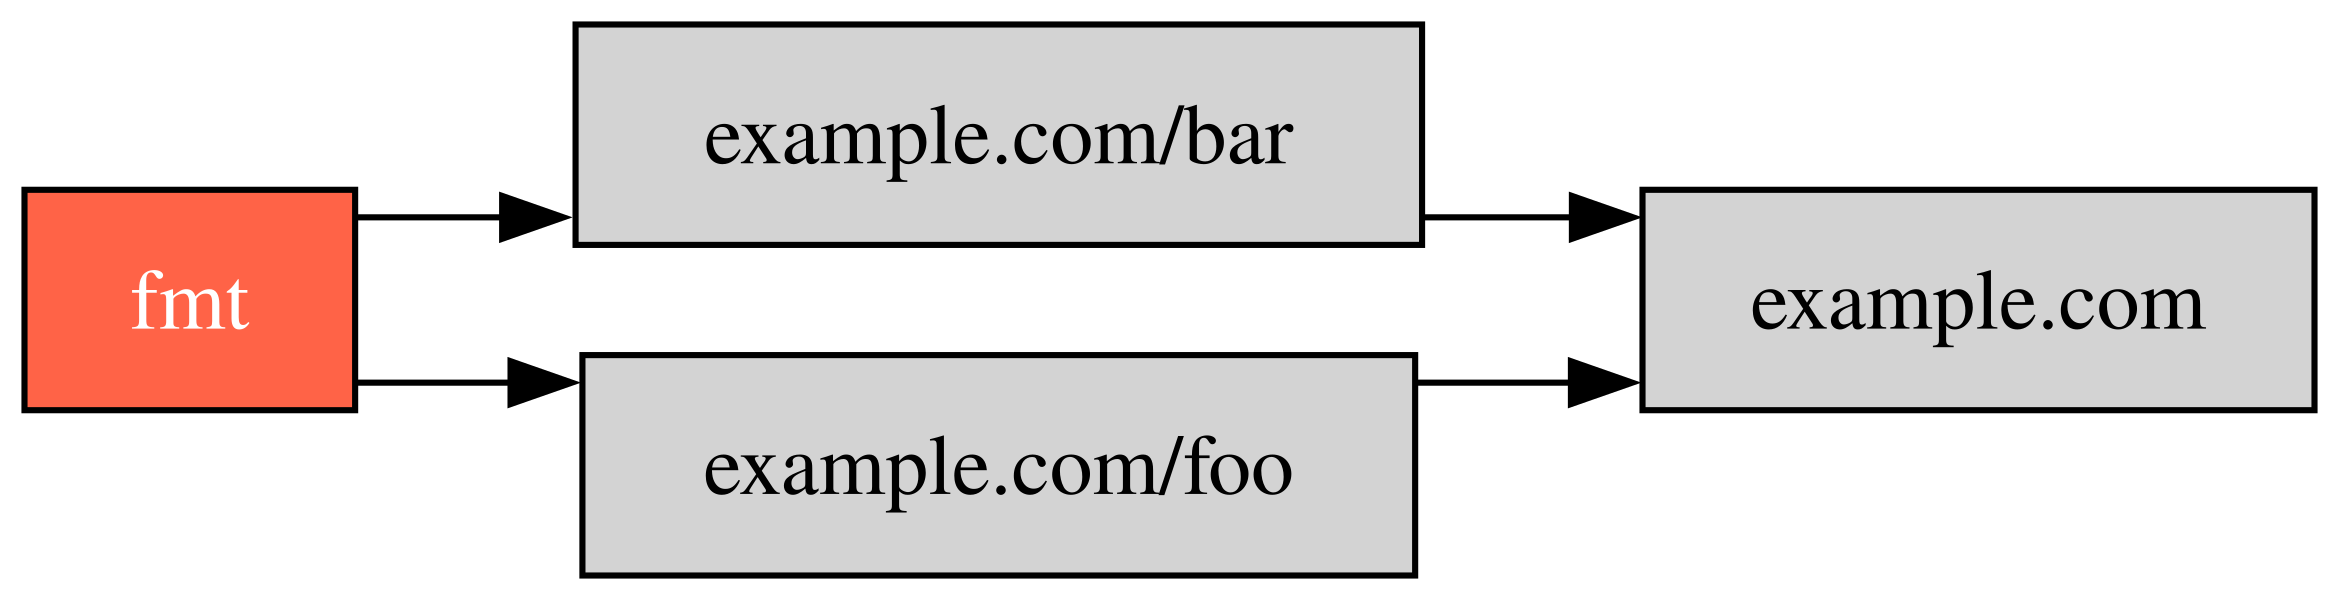
\includegraphics[width=1\textwidth]{examples/example.com.png}
\caption{Visualização do grafo de dependências gerado para o exemplo simples. Os nós em vermelho representam pacotes externos/padrão.}
\label{fig:grafoExemplo}
\end{figure}

\begin{figure}[ht]
\centering
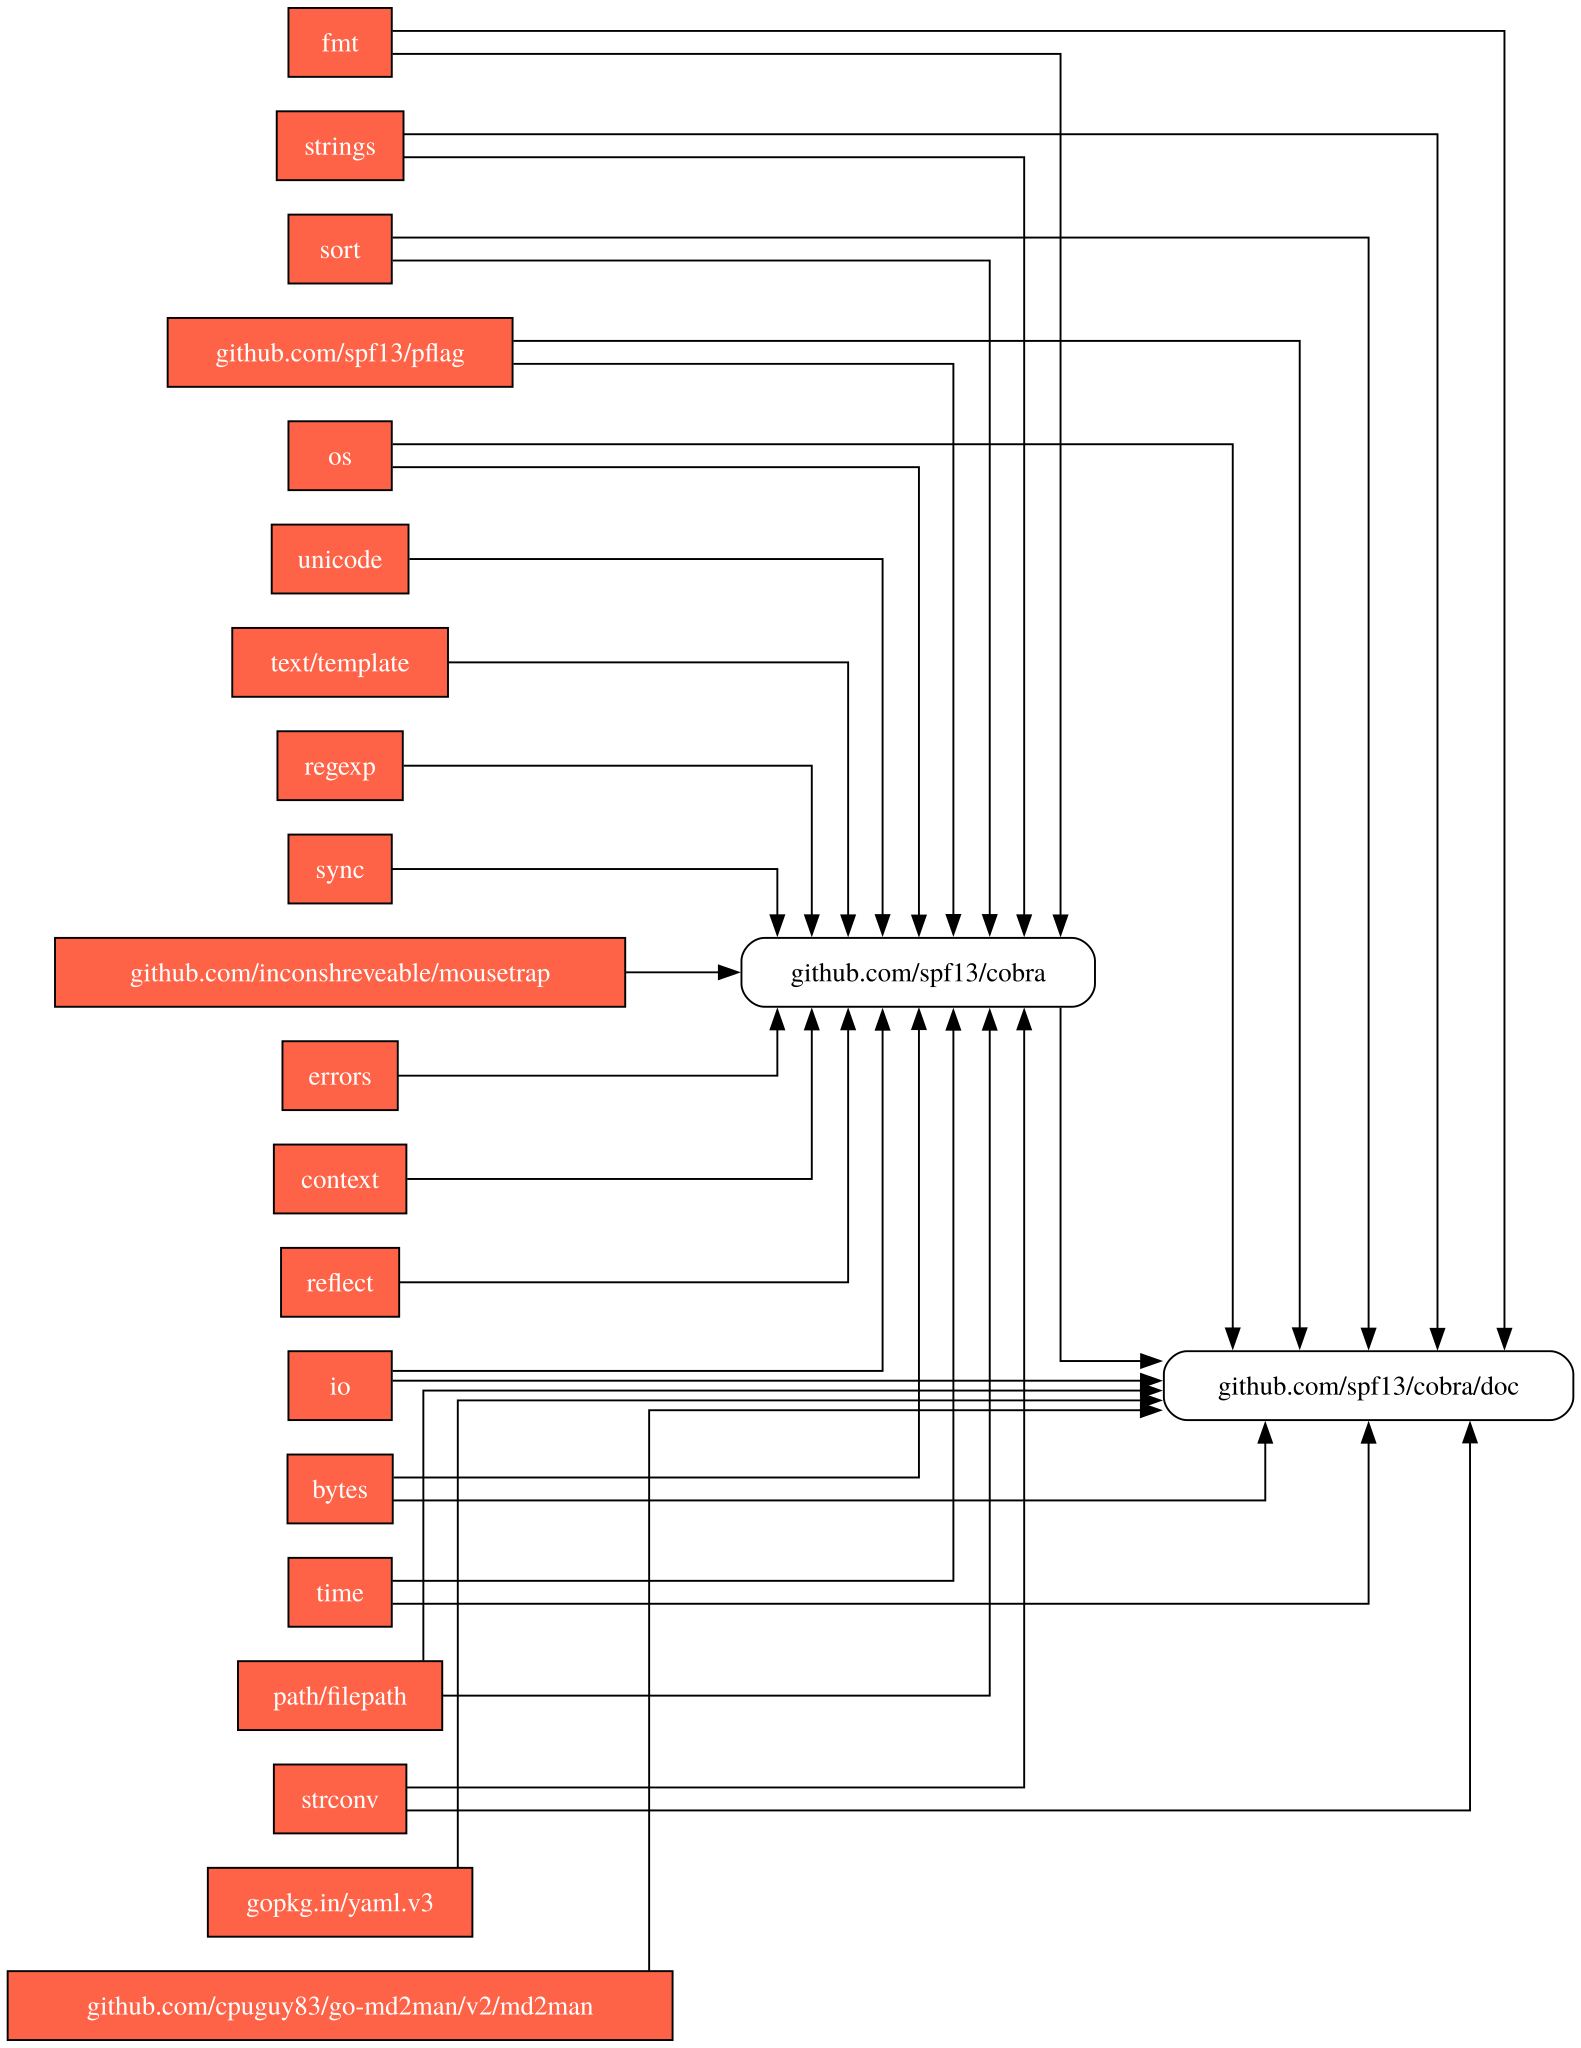
\includegraphics[width=1\textwidth]{examples/github.com_spf13_cobra.png}
\caption{Exemplo 2}
\label{fig:exemplo-2}
\end{figure}

\begin{figure}[ht]
\centering
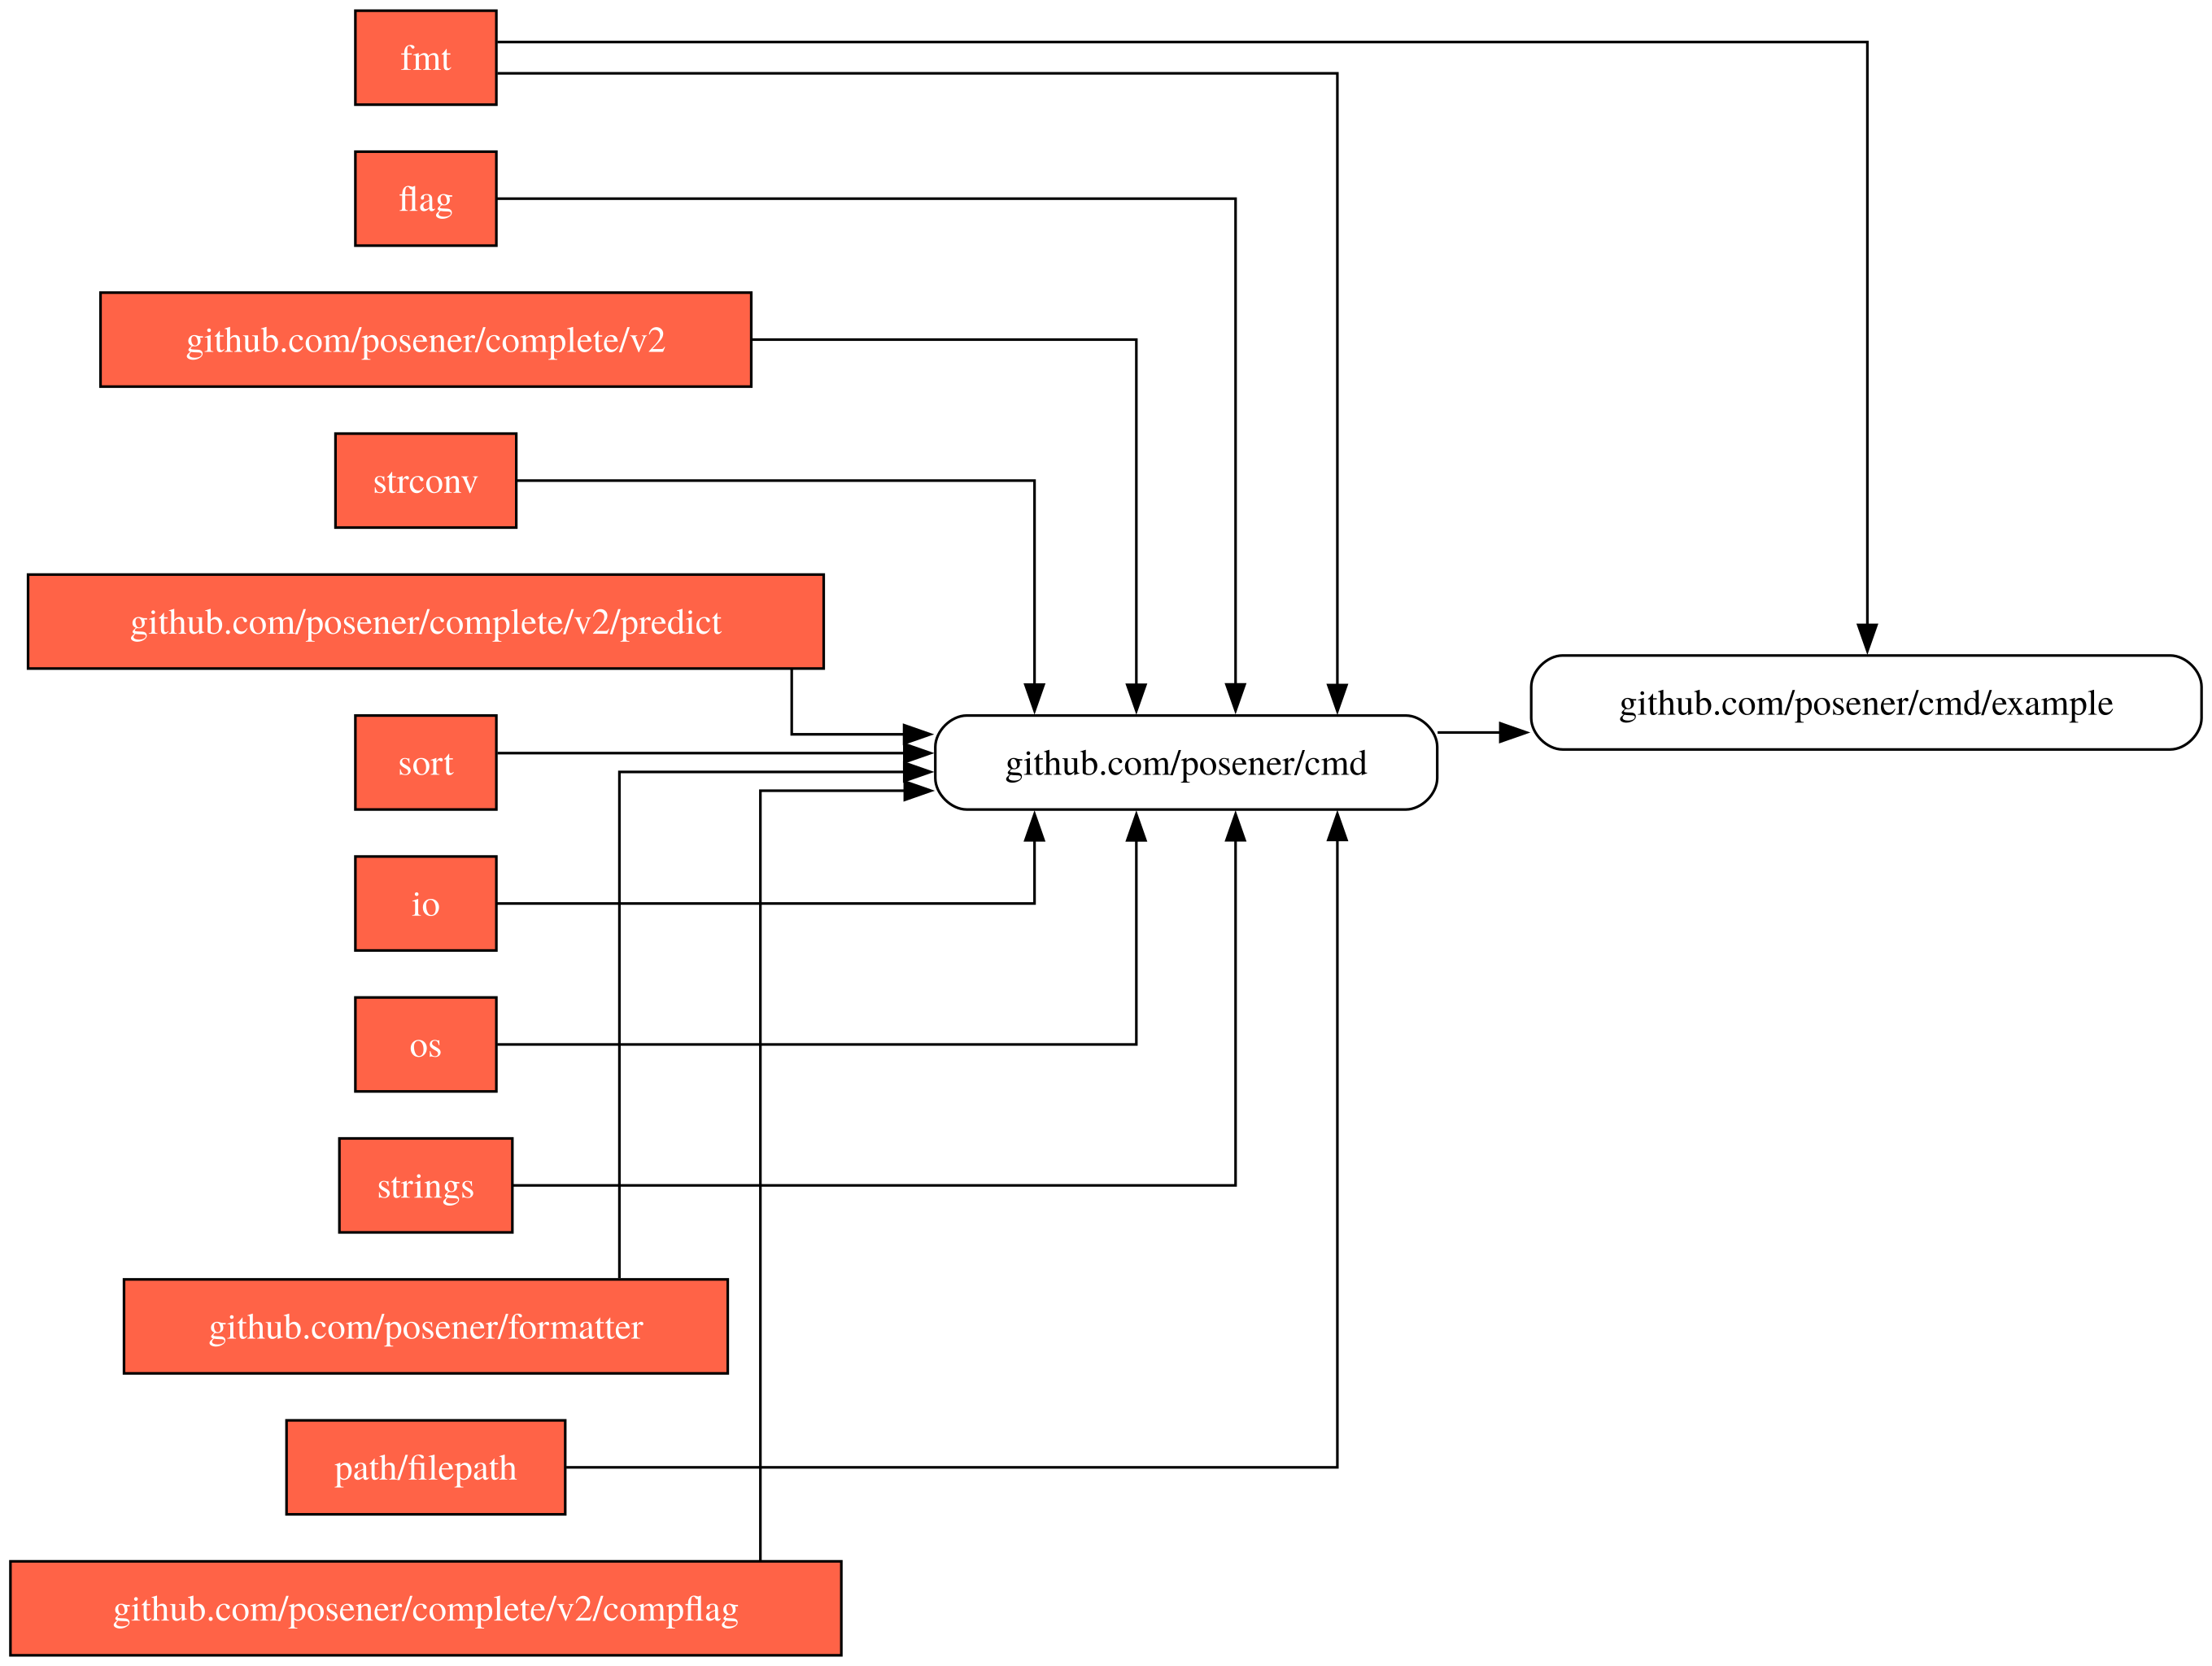
\includegraphics[width=1\textwidth]{examples/github.com_posener_cmd.png}
\caption{Exemplo 3}
\label{fig:exemplo-3}
\end{figure}

A clareza da visualização (Figura \ref{fig:grafoExemplo}) e a ordem explícita dos pacotes fornecem ao desenvolvedor uma visão imediata da arquitetura do projeto, facilitando a depuração de problemas de inicialização e a compreensão do fluxo de compilação.

\section{Conclusão}

Este trabalho apresentou uma solução computacional para o problema de gestão de dependências em projetos Go, alinhado aos objetivos da disciplina de Ferramenta de Processamento de Dados com Grafos. A modelagem do sistema de pacotes como um grafo direcionado provou-se eficaz, e a aplicação da ordenação topológica através do algoritmo de Kahn \cite{kahn1962} permitiu não apenas determinar a sequência de compilação segura, mas também estruturar a visualização dos resultados de forma intuitiva.

A ferramenta desenvolvida cumpre com sucesso os requisitos propostos: ela analisa o código-fonte, constrói um modelo em grafo, processa-o com algoritmos relevantes e apresenta os resultados de forma clara. A capacidade de detectar ciclos de dependência antes da compilação é um recurso valioso para evitar erros comuns em projetos de grande porte.

\subsection{Trabalhos Futuros}
Apesar de funcional, a ferramenta atual pode ser estendida de várias maneiras. Como trabalhos futuros, sugere-se:
\begin{itemize}
    \item \textbf{Análise de Desempenho:} Testar a ferramenta em repositórios de código aberto extremamente grandes (e.g., Kubernetes, Docker) para avaliar sua performance e escalabilidade.
    \item \textbf{Parser Avançado:} Substituir as expressões regulares por um parser de Abstract Syntax Tree (AST) da linguagem Go, o que tornaria a extração de importações mais robusta e precisa.
    \item \textbf{Integração com IDEs:} Desenvolver um plugin para editores de código populares, como o Visual Studio Code, que exiba o grafo de dependências e alerte sobre ciclos em tempo real.
    \item \textbf{Análise de "Peso" das Arestas:} Estender o modelo para incluir métricas nas arestas, como o número de funções ou tipos utilizados de um pacote dependente, para identificar acoplamentos fortes.
\end{itemize}

\bibliographystyle{sbc}
\bibliography{sbc-template.bib}

\end{document}
